\documentclass[12pt]{article}
\usepackage[margin=0.75in]{geometry}
\usepackage{float}
\usepackage{multicol}
\usepackage{lmodern}
\usepackage{amssymb,amsmath}
\usepackage{ifxetex,ifluatex}
\usepackage{fixltx2e} % provides \textsubscript
\ifnum 0\ifxetex 1\fi\ifluatex 1\fi=0 % if pdftex
  \usepackage[T1]{fontenc}
  \usepackage[utf8]{inputenc}
\else % if luatex or xelatex
  \ifxetex
    \usepackage{mathspec}
    \usepackage{xltxtra,xunicode}
  \else
    \usepackage{fontspec}
  \fi
  \defaultfontfeatures{Mapping=tex-text,Scale=MatchLowercase}
  \newcommand{\euro}{€}
\fi
% use upquote if available, for straight quotes in verbatim environments
\IfFileExists{upquote.sty}{\usepackage{upquote}}{}
% use microtype if available
\IfFileExists{microtype.sty}{%
\usepackage{microtype}
\UseMicrotypeSet[protrusion]{basicmath} % disable protrusion for tt fonts
}{}
\usepackage{graphicx}
\makeatletter
\def\maxwidth{\ifdim\Gin@nat@width>\linewidth\linewidth\else\Gin@nat@width\fi}
\def\maxheight{\ifdim\Gin@nat@height>\textheight\textheight\else\Gin@nat@height\fi}
\makeatother
% Scale images if necessary, so that they will not overflow the page
% margins by default, and it is still possible to overwrite the defaults
% using explicit options in \includegraphics[width=3.5in][width, height, ...]{}
\setkeys{Gin}{width=\maxwidth,height=\maxheight,keepaspectratio}
\ifxetex
  \usepackage[setpagesize=false, % page size defined by xetex
              unicode=false, % unicode breaks when used with xetex
              xetex]{hyperref}
\else
  \usepackage[unicode=true]{hyperref}
\fi
\hypersetup{breaklinks=true,
            bookmarks=true,
            pdfauthor={Brandon LeBeau},
            pdftitle={PSQF 4143: Section 7},
            colorlinks=true,
            citecolor=blue,
            urlcolor=blue,
            linkcolor=magenta,
            pdfborder={0 0 0}}
\urlstyle{same}  % don't use monospace font for urls
\setlength{\parindent}{0pt}
\setlength{\parskip}{6pt plus 2pt minus 1pt}
\setlength{\emergencystretch}{3em}  % prevent overfull lines
\setcounter{secnumdepth}{0}

\title{PSQF 4143: Section 7}
\author{Brandon LeBeau}
\date{}

\begin{document}
\maketitle

\section{The Normal Distribution}\label{the-normal-distribution}

\begin{figure}[H]
\centering
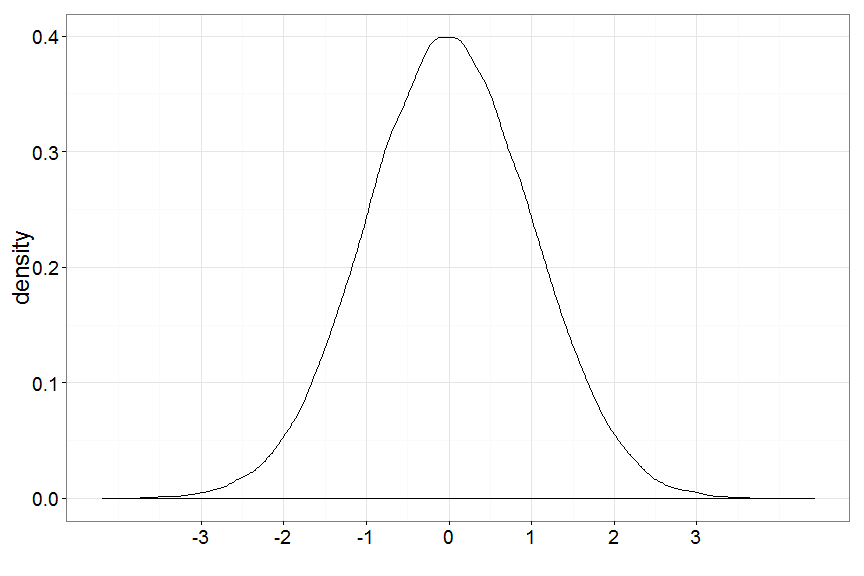
\includegraphics[width=3.5in]{figure/normal-1.png}
\caption{plot of chunk normal}
\end{figure}

\section{Normal Distribution History}\label{normal-distribution-history}

\begin{figure}[H]
\centering
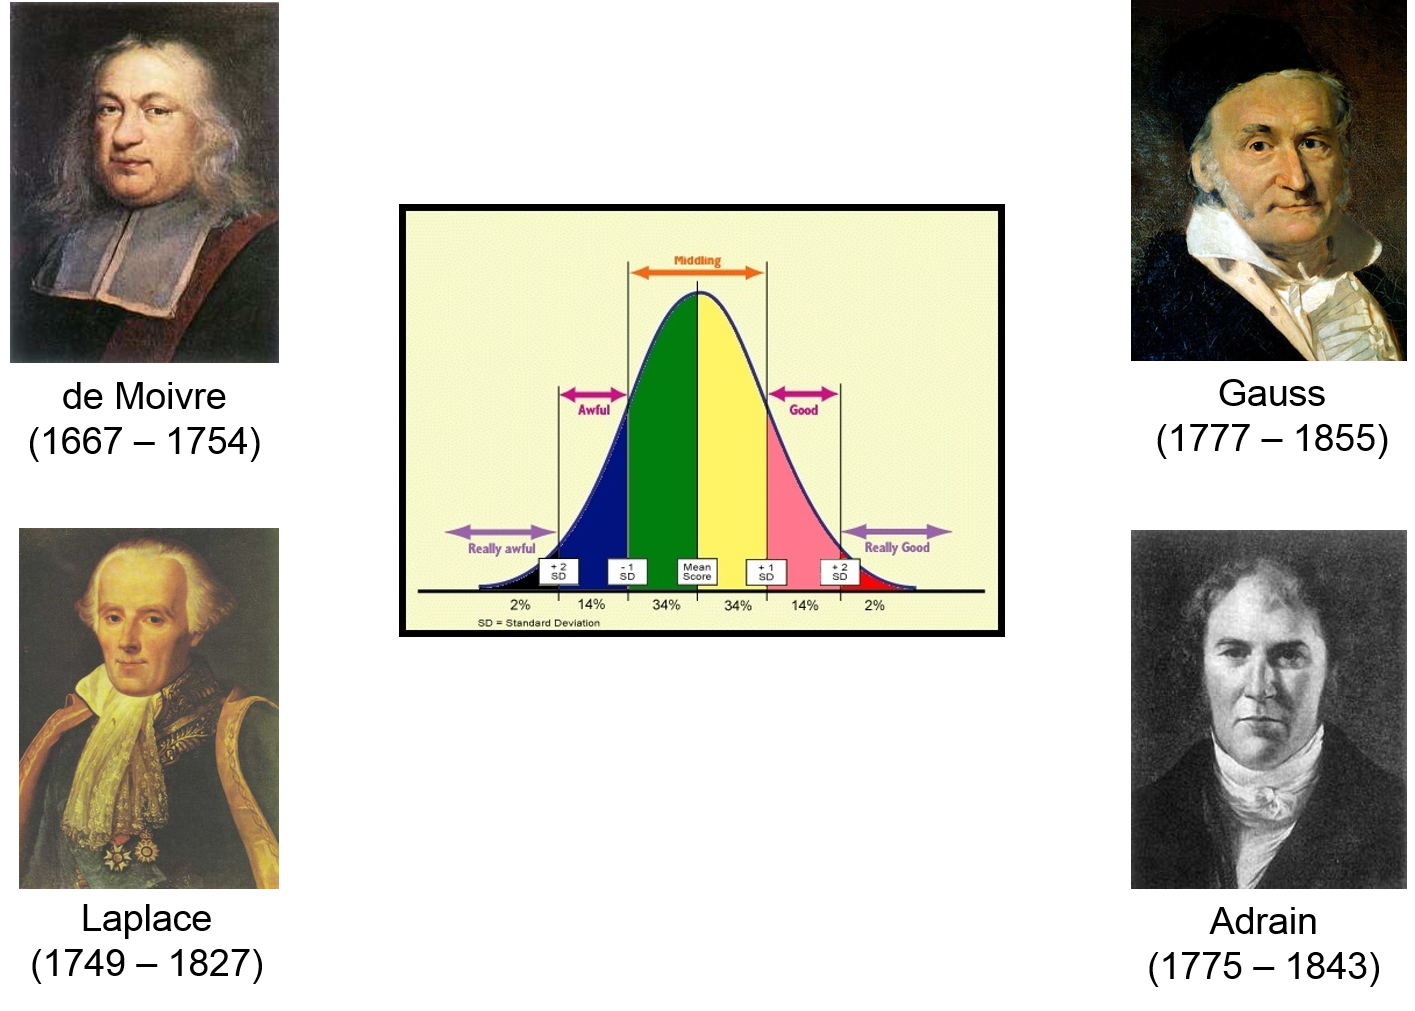
\includegraphics[width=3.5in]{normdist_people.png}
\caption{History}
\end{figure}

\section{Probability Models}\label{probability-models}

\begin{enumerate}
\def\labelenumi{\arabic{enumi}.}
\itemsep1pt\parskip0pt\parsep0pt
\item
  Equally-likely Model
\item
  Binomial Probability Model
\item
  Normal Probability Distribution

  \begin{itemize}
  \itemsep1pt\parskip0pt\parsep0pt
  \item
    As a model for real variables (section 7)
  \item
    As a model for sampling distributions (section 8)
  \item
    As a model for other probability distributions
  \end{itemize}
\end{enumerate}

\section{Properties of Continuous
Distributions}\label{properties-of-continuous-distributions}

\begin{enumerate}
\def\labelenumi{\arabic{enumi}.}
\itemsep1pt\parskip0pt\parsep0pt
\item
  The vertical axis does not represent probability
\item
  Probabilities are represented by areas under the curve
\item
  The total area under the curve is 1.
\item
  Can't talk about the probabilitly of a single score - always have to
  talk about ranges
\item
  Countinuous distributions that have means and standard deviations
  require calculus to computer
\end{enumerate}

\section{The Normal Distribution -
Mathematical}\label{the-normal-distribution---mathematical}

\[ Y = \frac{1}{\sigma \sqrt{2 \pi}}* e^{-\frac{(X - \mu)^2}{2 \sigma^2}} \]

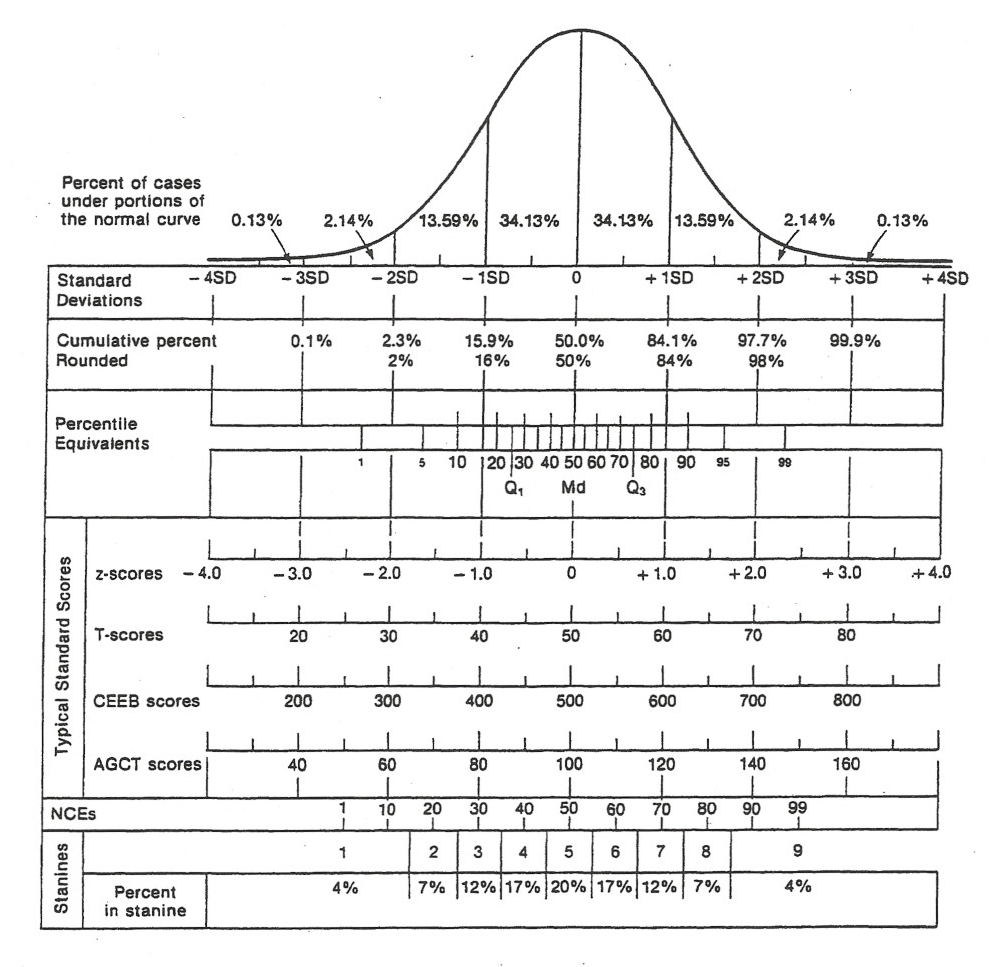
\includegraphics[width=3.5in]{standardscores.png}
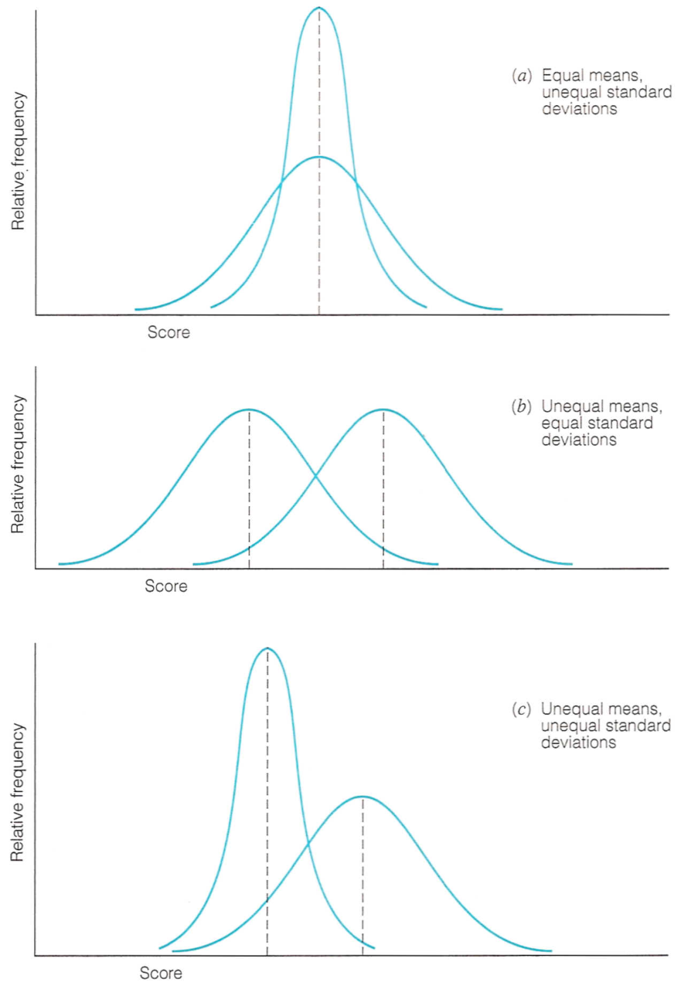
\includegraphics[width=3.5in]{normdist_different.png}

\section{Properties of The Normal
Distribution}\label{properties-of-the-normal-distribution}

\begin{itemize}
\itemsep1pt\parskip0pt\parsep0pt
\item
  Symmetric about the center of the distribution.
\item
  Mean, median, and mode are all equal.
\item
  Range: \(-\infty \leq X \leq \infty\)
\item
  The tails are asymptotic to the x-axis.

  \begin{itemize}
  \itemsep1pt\parskip0pt\parsep0pt
  \item
    i.e.~The tails get very close to the x-axis, but never touch it.
  \end{itemize}
\item
  The distribution has 0 skewness and kurtosis.\\
\item
  Very few scores greater than \(\mu + 3\sigma\)
\item
  The total area under any probability distribution regardless of the
  shape is 1.\\
\item
  We will use this fact in tandem with the mean and variation of a
  distribution to assign a probability of a specific value or mean.
\end{itemize}

\section{The Empirical Rule 1}\label{the-empirical-rule-1}

\begin{figure}[H]
\centering
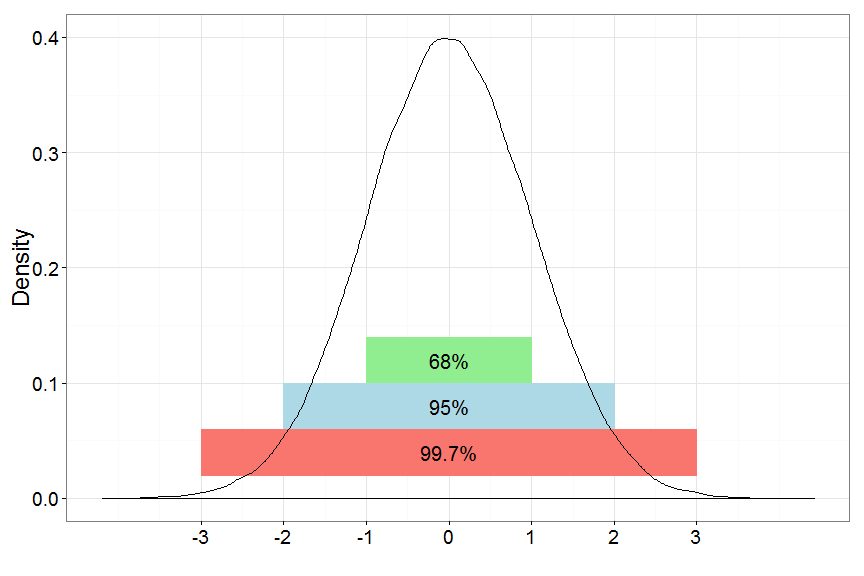
\includegraphics[width=3.5in]{figure/normal2-1.png}
\caption{plot of chunk normal2}
\end{figure}

\section{The Empirical Rule 2}\label{the-empirical-rule-2}

\begin{figure}[H]
\centering
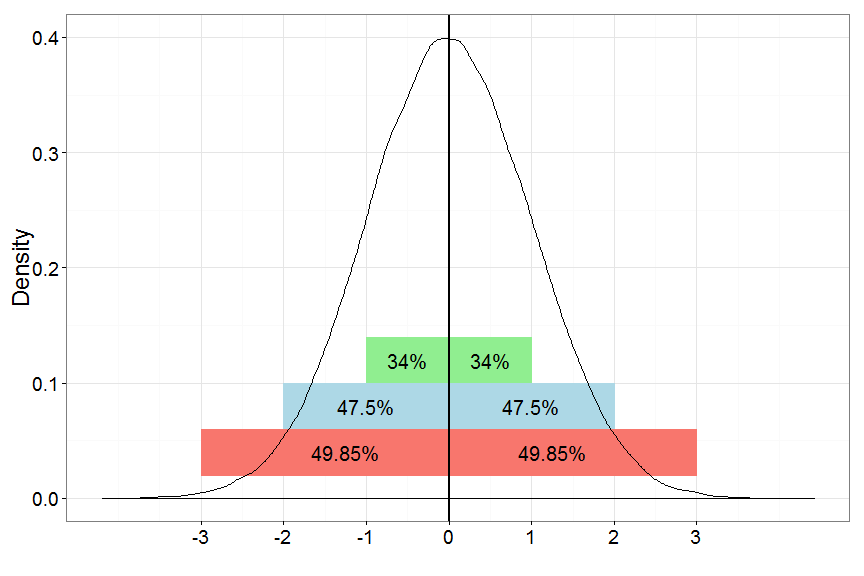
\includegraphics[width=3.5in]{figure/normal3-1.png}
\caption{plot of chunk normal3}
\end{figure}

\section{The Empirical Rule Summary}\label{the-empirical-rule-summary}

\begin{itemize}
\itemsep1pt\parskip0pt\parsep0pt
\item
  About 68\% of the data are within 1 standard deviation from the mean.
\item
  About 95\% of the data are within 2 standard deviations from the mean.
\item
  About 99.7\% of the data are within 3 standard deviations from the
  mean.
\end{itemize}

\section{Empirical Rule Examples}\label{empirical-rule-examples}

The average length of time a person stays at a job is 4.4 years with a
standard deviation of 1.8 years.

\begin{itemize}
\itemsep1pt\parskip0pt\parsep0pt
\item
  What percentage of employees stay on the job more than 6.2 years?
\item
  What percentage of employees stay on the job less than 0.8 years?
\item
  What is the probability of an employee staying at a job for more than
  9.8 years?
\item
  What is the probability of an employee staying on the job between 2.6
  and 6.2 years.
\item
  What is the probability an employee stays more than 7 years on the
  job?
\end{itemize}

\section{Standard Scores}\label{standard-scores}

\begin{itemize}
\item
  A \emph{z-score}, also called a standard score, is a way to represent
  a score in standard deviation units.
\item
  To compute a z-score: \[ z = \frac{X - \mu}{\sigma} \]
\item
  \(X\) is the raw score
\item
  \(\mu\) is the population mean
\item
  \(\sigma\) is the population standard deviation
\item
  A distribution of z-scores is also called the standard normal
  distribution.
\end{itemize}

\section{Standard Scores Examples}\label{standard-scores-examples}

The average length of time a person stays at a job is 4.4 years with a
standard deviation of 1.8 years.

\begin{itemize}
\itemsep1pt\parskip0pt\parsep0pt
\item
  Calculate the z-score and interpret it:

  \begin{itemize}
  \itemsep1pt\parskip0pt\parsep0pt
  \item
    \(X = 2.2\)
  \item
    \(X = 4.8\)
  \item
    \(X = 8.2\)
  \end{itemize}
\end{itemize}

\section{Using a z-table to find
probability/percentage/proportion.}\label{using-a-z-table-to-find-probabilitypercentageproportion.}

\begin{itemize}
\itemsep1pt\parskip0pt\parsep0pt
\item
  Answers the following types of questions:

  \begin{itemize}
  \itemsep1pt\parskip0pt\parsep0pt
  \item
    What proportion (probability/percentage) of the observations are
    less than/more than/between X years?
  \end{itemize}
\end{itemize}

\begin{enumerate}
\def\labelenumi{\arabic{enumi}.}
\itemsep1pt\parskip0pt\parsep0pt
\item
  Draw a normal curve, label the mean. Mark the value(s) of interest on
  the x-axis and shade the region of the curve corresponding to the
  region in question.
\item
  Convert the value(s) to a z-score.
\item
  Use the z-table to find the area below/above/between the calculated
  z-score(s).
\end{enumerate}

\section{How to use the z-table}\label{how-to-use-the-z-table}

\begin{figure}[H]
\centering
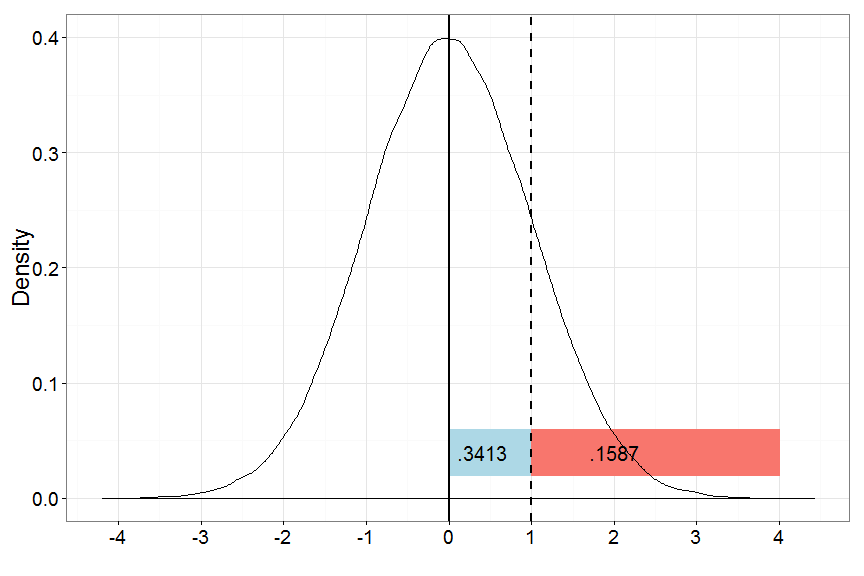
\includegraphics[width=3.5in]{figure/ztab-1.png}
\caption{plot of chunk ztab}
\end{figure}

\section{Z-table examples}\label{z-table-examples}

The average length of time a person stays at a job is 4.4 years with a
standard deviation of 1.8 years.

\begin{itemize}
\itemsep1pt\parskip0pt\parsep0pt
\item
  What is the probability an employee stays more than 7 years on the
  job?
\item
  What proportion of employees stay fewer than 4 years on the job?
\item
  What percentage of employees stay more than 5 years on the job but
  fewer than 8 years?
\end{itemize}

\section{Converting z-scores to a raw
score}\label{converting-z-scores-to-a-raw-score}

\begin{enumerate}
\def\labelenumi{\arabic{enumi}.}
\itemsep1pt\parskip0pt\parsep0pt
\item
  Multiply z-score by standard deviation.
\item
  Add the mean to the result from step 1.\\\(X = z*s + \bar{X}\)
\end{enumerate}

Examples: - \(Z = 1.25\) - \(Z = -.7\) - \(Z = 2.12\)

\section{Using the z-table to find a
value}\label{using-the-z-table-to-find-a-value}

What value of the variable is the cut point for the lower or upper
percentile?

\begin{enumerate}
\def\labelenumi{\arabic{enumi}.}
\itemsep1pt\parskip0pt\parsep0pt
\item
  Draw a normal curve, label the mean.
\item
  Mark the region of interest (upper or lower tail)
\item
  Use the z-table to find the z-score corresponding to the percentile
  region (area in the tail).
\item
  Convert the z-score back into the original metric (\(X\))
\end{enumerate}

\section{Examples}\label{examples}

The average length of time a person stays at a job is 4.4 years with a
standard deviation of 1.8 years.

\begin{itemize}
\itemsep1pt\parskip0pt\parsep0pt
\item
  How many years must an employee work at one job to be in the top 8\%
  of time at the job?
\item
  How many years must an employee work at one job to be in the bottom
  2\% of time at the job?
\end{itemize}

\section{More Examples}\label{more-examples}

\begin{itemize}
\itemsep1pt\parskip0pt\parsep0pt
\item
  In a normal distribution, what T-score is at the 15th percentile?
\item
  What percentage of the population has an IQ of 120 or higher?
\item
  What percent of scores are in the 6th stanine?
\end{itemize}

\section{More Practice}\label{more-practice}

The mean birth weight for infants is 7 pounds with a standard deviation
of 1.1 pounds.

Use the empirical rule to answer:\\1. What proportion of infants weigh
more than 8.1 pounds?\\2. What proportion of infants weigh less than 4.8
pounds?\\3. What proportion of infants are between 5.9 and 8.1 pounds?

Use the z-table to answer the following:\\1. What proportion of infants
weigh less than 5 pounds?\\2. What percentage of infants weigh more than
7.2 pounds?\\3. What proportion of infants weigh between 4.9 pounds and
7.1 pounds?\\4. How much would an infant weigh if they were in the top
12\%?\\5. How much would an infant weigh if they were in the bottom 4\%?

\end{document}
